\documentclass{usydthesis}

% Configuration

\def\degree{Master of Information Technology and Management}
\def\department{School of Information Technologies}

\title{{\bf\Huge Face Recognition on Fog Computing with the Capability of Scaling Out to the Cloud }}
\author{Chun Shen}
\def\sid{460317940}
\def\supervisor{Dr. Wei Bao}
%\def\assocsupervisor{Comment this line to remove assoc supervisor}

%%%%%%%%%%%%
% Packages

\usepackage{alltt}
\usepackage{amsfonts}
\usepackage{amsthm}
\usepackage[colorlinks=false,plainpages=false,a4paper,pdfborder={0 0 0},backref=false]{hyperref}
\usepackage[all]{hypcap}
\usepackage{listings}
\usepackage{longtable}
\usepackage{multirow}
\usepackage{pdflscape}
\usepackage{pgf}
\usepackage{pifont}
\usepackage{qtree}
\usepackage[english,rounding]{rccol}
\usepackage{rotating}
\usepackage{setspace}
\usepackage{style/bib}
\usepackage{subfigure}
\usepackage{tabularx}
\usepackage{tipa}
\usepackage{wrapfig}
\usepackage{xcolor}
\usepackage{xspace}
\usepackage{pgfplots}
\rcDecimalSignOutput{.} % rccol

\newenvironment{sidewaystablepage}{\begin{landscape}\begin{table}}{\end{table}\end{landscape}}

\def\subsectionautorefname{Section}
\def\subtableautorefname{Table}
\def\subfigureautorefname{Figure}
\def\chapterautorefname{Chapter}

\newcommand{\tick}{\ding{51}}
\newcommand{\cross}{\ding{53}}

\newcommand{\todo}[1]{{\color{red} #1}}
\newcommand{\sent}[1]{{\color{blue}\texttt{#1}\xspace}}


%%%%%%%%%%%%
% Maths functions
\def\O{\mbox{O}}

%%%%%%%%%%%%
% Setup

%   Page size:
\oddsidemargin=0cm	% really 1in
\evensidemargin=0cm
\textwidth=6.2677165in

\pgfplotsset{width=10cm,compat=1.9}

% initial page numbers:  i, ii, iii, ...
\renewcommand{\thepage}{\roman{page}}

\newcommand{\defn}[1]{\textit{#1}}
\newcommand{\ttl}[1]{\textit{#1}}
\newcommand{\txt}[1]{\textsf{\smaller #1}}
\newcommand{\qu}[1]{\textsf{#1}}
\newcommand{\txtbf}[1]{\textsf{\textbf{\small #1}}}
\newcommand{\quot}[1]{\textit{#1}}

\newcommand{\sssection}[1]{\textsf{\textbf{#1}}}

\newcommand{\cf}[1]{\mbox{$\it{#1}$}}   % category font

\newcommand{\alta}{\textsc{alta}\xspace}
\newcommand{\api}{\textsc{api}\xspace}
\newcommand{\candc}{C\&C\xspace}
\newcommand{\ccg}{\textsc{ccg}\xspace}
\newcommand{\ccgbank}{CCGbank\xspace}
\newcommand{\cky}{\textsc{cky}\xspace}
\newcommand{\jhu}{\textsc{jhu}\xspace}
\newcommand{\lfg}{\textsc{lfg}\xspace}
\newcommand{\hpsg}{\textsc{hpsg}\xspace}
\newcommand{\mwe}{\textsc{mwe}\xspace}
\newcommand{\mwes}{\mwe{}s\xspace}
\newcommand{\NE}{\textsc{ne}\xspace}
\newcommand{\Naive}{Na\"{i}ve\xspace}
\newcommand{\naive}{na\"{i}ve\xspace}
\newcommand{\ngram}{$n$-gram\xspace}
\newcommand{\ngrams}{\ngram{}s\xspace}
\newcommand{\nlp}{\textsc{nlp}\xspace}
\newcommand{\np}{\textsc{np}\xspace}
\newcommand{\nps}{\np{}s\xspace}
\newcommand{\parseval}{\textsc{parseval}\xspace}
\newcommand{\pos}{\textsc{pos}\xspace}
\newcommand{\pp}{\textsc{pp}\xspace}
\newcommand{\qa}{\textsc{qa}\xspace}
\newcommand{\ram}{\textsc{ram}\xspace}
\newcommand{\rasp}{\textsc{rasp}\xspace}
\newcommand{\tbl}{\textsc{tbl}\xspace}
\newcommand{\ptb}{\textsc{ptb}\xspace}
\newcommand{\wsj}{\textsc{wsj}\xspace}

\newtheorem*{definition}{Definition}
\newtheorem*{assumption}{Assumption}
\newtheorem*{mainassumption}{Main Assumption}
\newtheorem*{corollary*}{Corollary}




%%%%%%%%%%%%
% Start

\begin{document}

%%%%%%%%%%%%
% Title page
\maketitle

\setstretch{1.5}

% intro pages
\cleardoublepage
\phantomsection
\chapter*{Student Plagiarism: Compliance Statement} \label{sec:plagiarism}
{
\setlength{\parindent}{0cm}
\setlength{\parskip}{1em}

I certify that:   

I have read and understood the University of Sydney Student Plagiarism:  Coursework Policy and Procedure;

I understand that failure to comply with the Student Plagiarism: Coursework Policy and Procedure can lead to the University commencing proceedings against  me for potential student misconduct under Chapter 8 of the University of Sydney  By-Law 1999 (as amended);  

This Work is substantially my own, and to the extent that any part of this Work  is not my own I have indicated that it is not my own by Acknowledging  the Source of that part or those parts of the Work.  
}

\vspace{4cm}
\begin{tabular}{llll}
\textbf{Name}: & \authors & &  \\[2em]
\textbf{Signature}: & \hspace{0.4\textwidth} & \textbf{Date}: & \hspace{0.4\textwidth}\\[2cm]
\end{tabular}




\cleardoublepage
\phantomsection
\chapter*{Abstract}

The abstract goes in here.



\cleardoublepage
\phantomsection
\chapter*{Acknowledgements}

The thanks go in here.



% tables
\cleardoublepage
\setcounter{tocdepth}{2}
\tableofcontents

{\makeatletter
\renewcommand*\numberline[1]{\hb@xt@\@tempdima{#1 \hfil}\hspace*{1em}}
\makeatother
\listoffigures
\listoftables
\cleardoublepage
}

%%%%%%%%%%%%
% Chapters
\setcounter{page}{1}
\setcounter{chapter}{0}

% main page numbers:  1, 2, 3, ...
\renewcommand{\thepage}{\arabic{page}}	
\setupParagraphs

\chapter{Introduction}
The "pay-as-you-go" Cloud Computing model has dominated the private data centres market when it comes to web applications and batch processing\cite{bonomi2012fog}. The phenomenon is not out of expectation since Rajkumar Buyya predicted that the Cloud Computing was going to become one of the utilities namely water, electricity, gas and telephony in 2008\cite{buyya2009cloud}. Various modes of Cloud Computing are discussed with the perspective of business as well as appropriate algorithms based on these strategies. Paas, Iaas, SaaS are big names among them.

The world is not static. With the emerging devices connected to the Internet, generating data and asking for intelligent analysis, the burden of Cloud Computing increase sharply. As the data created through the Internet of Things(IoT) is expected to exceed counterparts of human beings, the single layer of Cloud Computing model is challenged \cite{vaquero2014finding}. Latency-sensitive applications get influenced heavier.

Bonomi et al., Cisco researchers, coined a term Fog Computing, tried to through light on this issue. In their concept, a middle layer called fog layer is introduced between the cloud(server-side) and end users(client-side). They argue that this three-layer mechanism may be the antiseptic solution of prosperous IoT. The aim of low latency will be achieved with the bonus of location awareness.

Potential scenarios where the Fog Computing mode shines attract researchers' interests. Given the trend of the rising volume, velocity and various data flow, real-time data analysis and relevant machine learning tasks are paid more attention. As a result, scenarios with the tag of "smart" such as Smart City, Smart Health, Smart Transportation gain popularity \cite{madsen2013reliability}.

Face identification, including face detection and face recognition, is predicted to be in high demand among these smart scenarios. So a Fog Computing based face identification should be proposed to fill in the gap. Considering the limited power of computing and battery, Fog Nodes in the architecture cannot handle the whole traffic alone; Cloud Nodes involve accordingly. A combination model of Fog Nodes and Cloud Nodes is formed, which offers end users a transparent computing layer where the location of the computing is unknown to them.

\chapter{Background} \label{chap:background}

\section{Inception of Fog Computing}
The inception of Fog Computing comes with the paper published by Bonomi et al. In that paper they discuss a relatively new computing paradigm based on the platform of internet of Things. In this paradigm, an extra layer is inserted between the cloud level and end devices level while this layer is not that close to these devices like Edge Computing units but reside a bit more far away in a more centralised way.  \cite{roman2018mobile} 

\section{Charactistics of Fog Computing}
Bonomi et al. emphasise that Fog Computing is not a substitute of Cloud Computing but an extension. They coined this concept based on the fact that the increasing demand of computing for automatically created data within IoT network. The following characteristics can be regarded as initial motivation of Fog Computing\cite{bonomi2012fog}:
\begin{itemize}
    \item Low latency and location awareness
    \item Wide-spread geographical distribution
    \item Mobility
    \item Very large number of nodes
    \item Predominant role of wireless access
    \item Strong presence of streaming and real time applications
    \item Heterogeneity
\end{itemize}

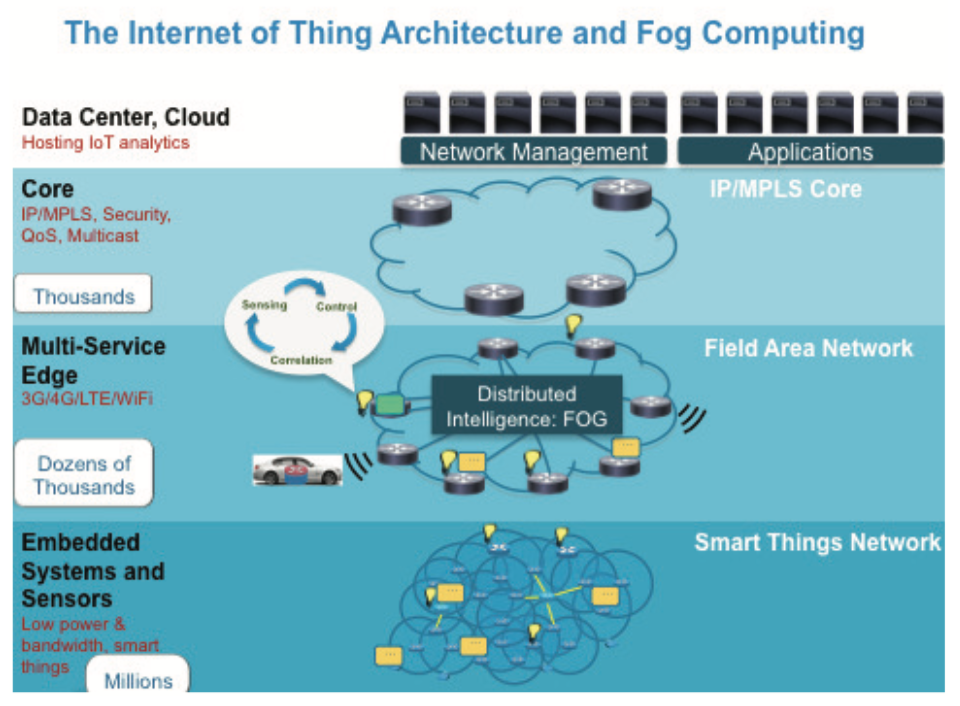
\includegraphics[width=\textwidth]{images/the_internet_of_thing_architecture_and_fog_computing.png}

\section{Scenarios of interest}

\subsection{Connected Vehicle}
Bonomi et al.\cite{bonomi2012fog}illustrate a smart traffic light system may become an suitable case applying the Fog Computing. They depict that cars are connected through local network receiving traffic support service, The connection can be via Wi-Fi, 3G, LTE, roadside units and light. In this case, there is a demand that traffic data is under real-time analysis and offer feedback correspondingly, which leading to the requirements of low latency. The high speed of vehicle intensify the significance of location awareness as well because the algorithm without overall optimisation may provide better speed performance.

\subsection{Smart Grid}
Smart grid borrows strength from Fog Computing either. The data generated by grid sensors and devices can get processed at the first tier of the Fog, called machine to machine interaction. The rest part of the layers provide analytic functionality of big data processing. 

\subsection{Wireless Sensor and Actuators Networks}
Wireless Sensors nodes are designed as an extremely low power devices, which may benefit from the shared computing capability via fog nodes. All relevant energy constrained devices are considered as advocates of the similar concept.

\subsection{Smart Building}
Beside three scenarios discussed in the paper written Bonomi et al.\cite{bonomi2012fog}, Stojmenovic et al. complement two other secnatios.\cite{stojmenovic2014fog} Smart building is one of them.

In the scenario of Smart Building, temperature, humidity and relevant environment measurements are collected and interact with each other via higher level fog node.

\subsection{Software Defined Network}
With SDN gaining more attention, studies based on it expanded to the area of Fog Computing. Stojmenovic et al. explain the Fog Computing can be used in vehicular network to apply the concept of Software Defined Network since it helps separate control and data communication layers. Furthermore, lack of communication among peers in vehicular network make Fog Computing a remedial solution when it comes to high packet loss rate.\cite{stojmenovic2014fog} 

\subsection{Augmented Reality}
Yi et al.\cite{yi2015survey} introduce more realistic scenarios in their paper and real-time video analytic is one of them. They consider the popularity of Augmented Reality products such as Google Glass and Microsoft HoloLens that demand high computation power. AR applications notoriously rely on the processing capability of hardware. Multiple sources of media are going to combined and calculated simultaneously. What's more, even a bit of latency can be sensed by users and eventually impact the outcome. On the other side, intensive computing tasks consume enormous energy, make the mobility of AR hardware unavailable. 

Fog Computing can be plugged to this case. Since we do not push the computing nodes far away from the data, the latency can be ensured. Meanwhile, it saves the power of the devices because these power-consuming tasks are diverted to external hardware and only basic network I/O is contained.

\subsection{Content Delivery and Caching}
Zhu et al. contribute to another scenario of Fog Computing. In their paper, Fog Computing nodes are used as Content Delivery Network nodes. They believe that most of time wasted in the front-end rendering and execution can be saved if cache is optimised and static resources are better compressed. Their concept of Fog Computing is higher level of Edge Computing. In other words, Fog Computing nodes are more centralised and offer the bridge between cloud and end users. In the scenario, the end users are equipped with computing power to some degree and are not as power sensitive as nodes in wireless network. As a result, higher level of Fog Computing nodes play the role of distributed tasks of Cloud Computing. They help preprocess web objects, page components and minimise traffic.

\subsection{Mobile Big Data Analytic}
The same authors also mention the significance of Fog Computing in the scenario of big data processing. Consider the high demand of Cloud Computing as the resource of big data analysis, relevant tasks pop up dramatically. Sometimes, the Cloud Computing node are far away from end users and low latency top the requirement, Fog Computing nodes become decent alternative. In this use case, Fog Computing strengthen their feature of elasticity and scalability just like the Could counterpart.
\chapter{Related Work} \label{chap:relatedwork}


\section{Mobile-Cloudlet-Cloud Acceleration Architecture (2012)}

Soyata et al. proposed architecture of mobile-cloudlet-cloud in 2012. They found that face identification techniques are demanded everywhere such as airport security, law enforcement and cover a series of stages \cite{soyata2012cloud}. Image extracting and re-sizing, feature extractions and detection are core components among these stages, which relies on intensive computation.

Given low power of computing and limited bandwidth of end devices, they make use of cloudlet to execute pre-processing tasks. For example, they extracted Haar features instead of sending the whole image to the cloud to reduce network consumption. On the other hand, this feature extraction tasks are allocated to underlying cloudlets, so that burden of the Cloud Computing is lessened.

\section{Mobile Cloud Computing (2014)}

Ayad et al. articulated the emerging research topic of face recognition in their paper published in 2014. They regarded facial identity as useful crime-fighting tools. The increasing number of mobile devices also attract their attention, most of which embeds decent image capture hardware. To the contrary, the computing power of these mobile devices is incompetent to analyse the collected data. Authors drafted a concept of mobile cloud computing to break this situation. 

Various cloud computing models are discussed in their paper with private cloud highlighted. OpenStack and OpenShift are considered in this cloud deployment model \cite{ayad2014real}. Furthermore, they covered the previous definition of the mobile cloud computing model, to be specific, three. Soyata et al.'s work is referred when they tried to include experience as much as possible.

After investigating mainstream face detection and recognition technologies, nothing newer introduced. However, these authors took relevant issues of security and trust into consideration.

\section{Fog Computing Based Face Identification (2017)}

Hu et al. presented a fog-based model for face identification in 2017 based on the fact that identification technology is prerequisite for consistency of physical-cyber space mapping in the Internet of Things \cite{hu2017fog}. Given face is a distinctive feature of human, they conduct their experiment through it. 

In their prototype system, fog computing nodes are taken responsibility for image pre-processing and feature extraction tasks just as the cloudlet does in Soyata et al.'s paper. The cloud nodes only play the role of face detection and recognition. Relevant face matching algorithm is LBP that is a traditional face recognition method.
\chapter{Contribution} \label{chap:contribution}

Even though much work has been done according to the discussion in the previous chapter. These related work may not preciously reflect the fast pace of march in the field of hardware. The overall computing power is continuously advancing. In the case of Internet of Things, power of nodes deployed in various scenarios also boosts without hesitation. Tasks that used to be not suitable for nodes in the Internet of Things now become common ones. 

Based on this fact, I propose an aggressive model where more tasks are offloaded from cloud nodes to fog nodes to further lower network latency. Due to vague outcome of this adjustment, performance of various aspects of the system will be measured. As a result, a matrix should form to prepare raw data for further analyse.

On the other hand, Fog nodes in this architecture are not to substitute the Cloud Nodes completely. Considering the constrained power consumption, low unit computing price of cloud and elasticity of cloud infrastructure, tasks failing to be digested in the Fog layer will be overflowed to the cloud. So a relevant mechanism is drafted to dynamically allocate the tasks among Fog Nodes and Cloud Nodes

My contribution to this topic can be split into three parts:
\begin{itemize}
    \item A Fog Computing model with a prototype where face identification tasks are finished closer to end devices. The prototype of this model is implemented to evaluate the performance.
    \item A draft of dynamic allocation mechanism to judge where the face identification should be executed.
   \item A form of a transparent computing model based on the combination of the Cloud and Fog Nodes.
\end{itemize}

\section{Fog Computing based Face Identification}
As we discussed, the power of Fog nodes is increasing so that it can handle more computing tasks rather than just pre-processing tasks. In my architecture, computing of face detection and recognition is finished in the Fog Nodes. When these nodes find follow-up workload is beyond their capability, a dynamic allocation mechanism will be triggered to coordinate schedules of ambient Fog nodes or involved Cloud nodes. 

\section{Performance Evaluation of current computing model}
Considering that offloading workload from Cloud Nodes to Fog Nodes may lead to changes on various grounds, performance benchmarks should be set up to evaluate whether the merits outweigh the demerits.

\section{Dynamic Allocation Mechanism}
As mentioned in the section above, there is an mechanism used to overcome the potential overload of Fog Nodes. This mechanism helps calculate the required number of Fog Nodes based on prior traffic and support where to locate the computing nodes. Proxy techniques are assumed to be used to direct the request from end devices to target computing nodes.

\section{Transparent Computing Model}
\chapter{Design of the System} \label{chap:design}
This chapter is about the design of the system. It covers the components I used in the Fog Computing based face identification system and explain the reason why I come to this idea. Then, the next chapter will give more practical implementation detail of this design.

\section{Overview}
On the whole, the system consists of two behaviour mode, namely off-peak mode and peak mode. Off-peak mode means the requests from end devices are sparse or distributed evenly so that Fog Nodes own the capability of responding within a limited time slot. Cloud Nodes are not involved in this mode. On the contrary, peak mode demands the power of Cloud Nodes. This mode is triggered through a dynamic allocation algorithm which monitors the pressure of the Fog Nodes.

\section{Off-peak Mode}
This mode only cover the lower two layers in the figure \ref{fig:design_of_the_system}. As you can see in the figure, the lowest layer contains end devices in the network of the Internet of Things. 

In my implementation, The Nexus 6 Android phone is used to play the role of the end device. Though there is only one android depicted in the figure, it is on behalf of all Internet of Things devices with limited hardware resource. This device is in charge of collecting images through preview frame from a camera and sending them to a closest working Fog Node periodically.

The Fog Nodes in the higher layer (medium layer) substitute the Cloud counterparts as the resource pool of computing. They are commodity personal computers in my implementation. They provide the service of face detection and face recognition. At the same time, they monitor the traffic of request to make the decision that whether Cloud Nodes should be included in the computing cycle and how many of them are required. This feature is called dynamic allocation in the system.

\section{Peak Mode}
Peak mode contains three layers as a whole. Compared to off-peak mode, one more layer is added. The top layer consists of Cloud Nodes, and the rest of layers are the same with the off-peak mode.

Peak mode is activated when the requests from the end devices are frequent. This mode involves Cloud Nodes, which make it different from the Fog mode. Amazon EC2 or other cloud computing infrastructures are used as an elastic resource pool. Due to its characteristic of elasticity, temporary high demand for computing tasks can be flattened.

Expected disadvantages of introducing the Cloud Nodes includes longer latency and security issues.

\section{Face Identification}
Face detection and recognition algorithm themselves are popular research topics. Consider they are not my focal topic, I tried to bring in popular implementations aimed at gain confidence for my system.

\begin{figure}
    \centering
    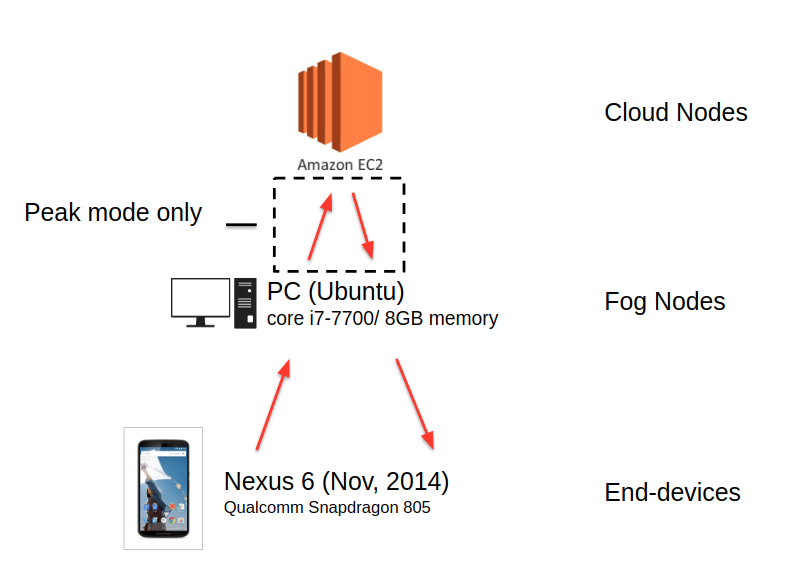
\includegraphics[width=0.7\textwidth]{images/design-of-the-system.png}
    \caption{Design of the System}
    \label{fig:design_of_the_system}
\end{figure}


\chapter{Implementation of the System} \label{chap:implementation}

The methods used to implement the system and relevant challenges raised are discussed in this chapter. Dedicated explanation of the technical specification can be found in this chapter as well. The explanatory sequence diagrams are illustrated to brief the workflow of the system at the end.

\section{Implementation on the Side of End Devices}

As mentioned in the chapter \ref{chap:design}, the end devices are simulated by android phones in my implementation. The  Internet of Things devices that play the role of sampling ambient information through a video format are assumed as weak computing devices. In other words, they follow the philosophy of design that more tasks are finished with less power and computing unit. The cost of them is low accordingly so that they are realistic for large-scale deployment.

\subsection{Android Devices}
Nexus 6 is used in the experiment, which was published in 2014, about four years ago. This phone is manufactured by Motorola and embedded with a Qualcomm 2.7 GHz quad-core Krait 450 CPU. \cite{wiki:nexus6} The power of this android phone is not as strong as mainstream counterparts such as Google Pixel 2 nowadays. This weakness contributes to its competence as the replacement of devices in the network of the Internet of Things.

\subsection{Operating System}
The operating system version of this android phone is 7.1.1 "Nougat"\cite{android-api}. API lever of this version is 15 while it is not compulsory since I make use of the android.hardware.camera2 API that is introduced in Android 5.0 (API level 21) \cite{android5.0}. This update enhances the control towards the camera so that fine-grain photos can be captured. 

\subsection{Image Capture}
The Android phone is equipped with both front and rear camera. The only rear camera is used to capture the video stream. The resolution of the sensor is 13MP \cite{wiki:megapixel}, however, I do not extract the image from the camera directly, so the resolution does not decide the final size of the image.

The process of my sampling the images is as follows. I make the application executed and turn the camera into preview mode in which camera continuously collect image frames and push to the surface view of the android application. Then another thread in the application manages to sample images from these surface view according to the frequency appointed. As a result, the resolution of the image is decided by the size of the screen which is about 2560 x 1440 px. The rate is adjustable according to the configuration.

The preview images will be compressed with PNG format  \cite{roelofs1999png} which is a lossless image compression format with broad compatibility among Internet. The quality level of the image is set to 90 per cent while the original image is reduced to half size. This help to decrease the pressure of network bandwidth.

\section{Network between End Devices and Fog Nodes}
In the previous part, the process of image collection is described. Since the face detection and recognition tasks are not arranged locally, they are assigned to the closest Fog Nodes.

The IP address of the Fog Node is hard-coded into the application so rigid network configuration should be followed to make the application to locate the corresponding Fog Nodes. Dynamic Host Configuration Protocol (DHCP) \cite{droms2002dhcp} is an ideal protocol to handle the gap, and actually, it is used in the experiment.

An appointed IP address remains for Fog Node deployment in every sub-network where Fog Node should be accessible. As the diagram \ref{fig:network} shows, end devices are connected to the Fog Nodes directly, within one hop ideally. The links between the Fog Node and Cloud Nodes in different sub-networks (dyed in four different colours) are various. This uncertainty contributes to the network latency in part.

\section{Communication between End Devices and Fog Nodes}
The network part shares the underlying physical implementation of the system, and this section covers the protocol used to transmit the collected image data to the Fog Nodes.

Considering Fog Nodes will be distributed into a heterogeneous network, compatibility of the protocol owns a high priority. Hypertext Transfer Protocol (HTTP) is among mainstream standards and play the role of De facto foundation for the World Wide Web \cite{fielding1999hypertext}. So I appoint it as the underlying protocol for the application layer in the Internet protocol suite, namely TCP/IP.

Two-way communication is suitable for the scenario. Schedulers sample images and send them to the Fog Nodes for face identification in a recurring way. The instant outcomes will be pushed back to original devices as soon as possible. The data flow of processes mentioned above go in opposite direction, reveal the feature of two-way communication. So the traditional request-response client-server protocol is wiped out from the options due to its disqualification.

The frequency of requests also damages the shine of the HTTP because of its tedious handshake stage. Even though HTTP/1.1 introduced a keep-alive-mechanism to reuse the previous connection for the incoming request, I prefer the emerging standard of full-duplex communication through HTTP.

WebSocket is a favourable protocol that supports two-way communication and removes the dependence upon multiple HTTP connections  \cite{fette2011websocket}. This mechanism is initially designed for carrying a short message between clients(mainly browsers) between servers. It sounds marvellous for building a real-time chat channel, especially when it comes to compatibility. WebSocket integrates itself with HTTP protocol and is built with TCP. The default port of it is 80, which add to its highlights \cite{fette2011websocket}.

According to the characteristic of WebSocket mentioned, pre-processing of the images is invoked. Considering encoding schemes supported by HTTP, binary data should be converted before they are put into the payload. Base64 is made use of to avoid the omission of the data with the explanation followed.

Base64 make underlying data can be delivered in a textual format to bypass specific legacy system or lead to better interoperability  \cite{josefsson2006base16}. In our case, it is needed to encode binary data before it is transported to the server side to keep the data intact. The code section in the figure \ref{fig:png_base64} displays how I do the image pre-processing through the Java SDK.

\begin{figure}
    \centering
    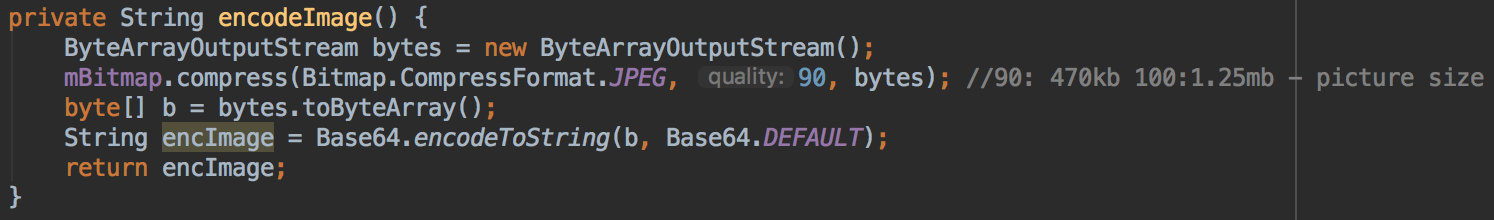
\includegraphics[width=\textwidth]{images/png&base64.png}
    \caption{Image Compress  Base64}
    \label{fig:png_base64}
\end{figure}



\begin{figure}
    \centering
    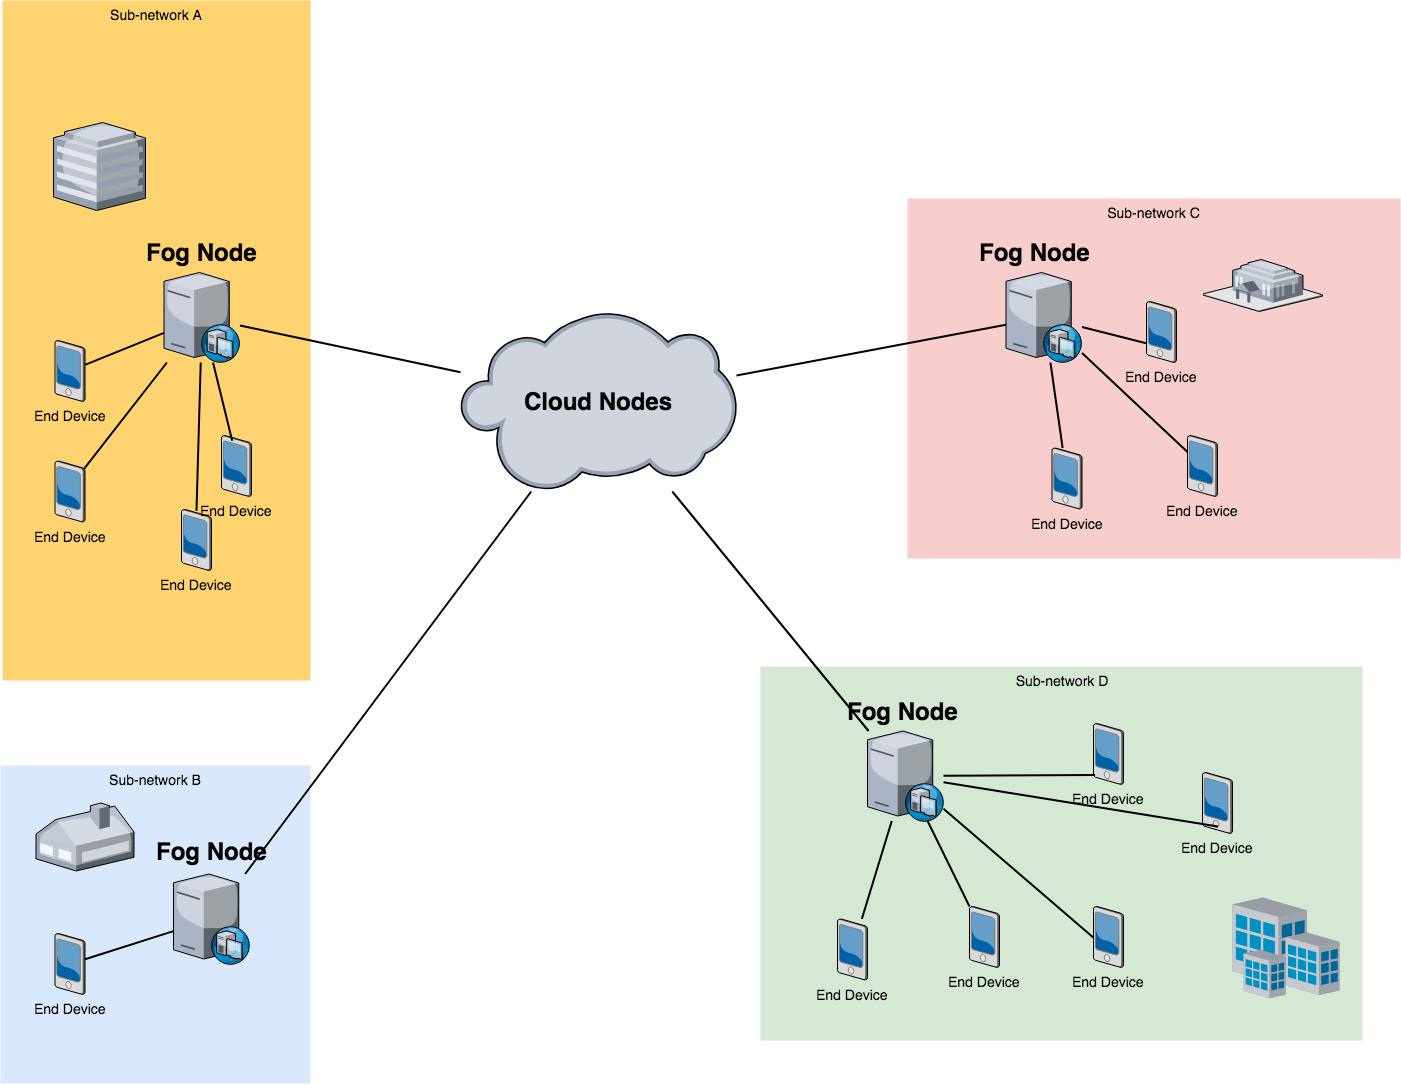
\includegraphics[width=\textwidth]{images/network.png}
    \caption{Network connection}
    \label{fig:network}
\end{figure}


\section{Implementation on the Side of Fog Nodes}
This section discusses the technical specification when it comes to building the corresponding Fog Nodes. The image pre-processing and data decoding processing are symmetric to the original one, so descriptions are briefed. Generally speaking, the images restore on the side of Fog Nodes, and WebSockets keep consuming incoming event with the payload of the image and respond accordingly.

The following subsections focus on two routines implemented for performance benchmarks. The difference between them is the algorithm of face identification.

\subsection{Fog Basic}
As displayed in the figure of \ref{fig:preview}, there is a button, the third button from the left, in charge of starting the mode of Fog Basic. In this mode, the face identification tasks will be sent to the port on the server with the basic face detection functionality. 

\subsubsection{Face Detection}
OpenCV provides solid face detection module called Haar Feature-based Cascade Classifiers \cite{opencv_library}. In their tutorial documentation, they underline that this classifier is an effective object detection method. This method is proposed by Paul Viola and Michael Jones and depicted as a machine learning based algorithm  \cite{viola2001rapid}. The algorithm extract features from the grey image and applies Adaboost to the virtually 160000+ features. Their paper argues 200 features offer the detection with 95\% accuracy. An idea of discarding regions without faces at an earlier stage is composed to improve the computing. This is the story behind classify the algorithm into Cascade of Classifiers.

Haar Feature-based Cascade Classifiers saves training stage in the implementation due to existing trained model for human faces and eyes. The XML classifier file can be found in their SDK under the name of "haarcascade\_frontalface\_default.xml".

To stream images decoded from the end devices to the face detection module, OpenCV image manipulation module is introduced. The relevant operations include recognising the compression format of the image, extracting RGB information from the image container and map the RGB colour space to the Grey space. Because colour metadata is unnecessary to Haar algorithm, grey images are prerequisite of this algorithm.

Node-opencv provides the OpenCV bindings for Node.js  \cite{node-opencv}. This third-party open source project is relied on to make the image stream interplay-able with the underlying native computing layer, namely OpenCV C++ native code.

\subsubsection{Web Server}
As discussed in the Communication section, WebSockets protocol is in use. Since it is just a protocol, it should be implemented by a certain programming language or specific framework. This section offer detail about the required web application container and its environment. 

Node.js is asynchronous event-driven JavaScript runtime targeting at scalable network applications \cite{nodejs}. In their official documentation, Node.js regards HTTP as a first class citizen which means it puts streaming and low latency in the heart. The predominant advantages of Node.js make itself an appropriate candidate when it comes to implementing WebSockets.

Among well known Github open source projects, Socket.io are gaining increasing popularity. This library features the fastest and most reliable real-time engine \cite{socketio}. It completely realises the standard of WebSockets and successfully builds the rich ecosystem around it. SDK offered range from browser environment to cross-platform mobile operating systems such as Android and iOS. Since its feature satisfied the requirement, it is used for Fog Basic mode as the middleware of the Web Server, running upon the Node.js runtime.

The node-opencv can be chained with the event handler of Socket.io, leading to saved context change and fewer data exchanges. Image data from end devices is collected and merged through Socket.io and handed over to the node-opencv simultaneously on the same Node.js runtime. 

\subsection{Fog DNN}
The button labelled with "Fog DNN" triggers another mode where deep learning based face recognition is used. You can see the button is located at the bottom centre of the figure \ref{fig:preview}.
The face identification algorithm computes the name of detected faces, other than just the location of the faces.  

\subsubsection{Face Recognition}
Compared to the prior mode of "Fog Basic", higher quality face identification tasks succeed in this mode. To be more specific, The Fog Basic mode only detects the location of the faces upon one image frame, while Fog DNN mode steps further. Fog DNN manage to match faces to known faces to report the name of that face.

The functionality of face recognition is delivered by Dlib. Dlib is developed by Davis King and start with the target of building a general purpose library in 2002 \cite{dlib09}. Considering the popularity of machine learning, contributors focus on the relevant tools as well. Deep metric learning tooling is added to the Dlib in recent releases.

Davis King, the contributor of the Dlib, implemented the ResNet network and imported it into the library last year. This model is an essential version of the ResNet-34 network which is proposed through the paper Deep Residual Learning for Image Recognition  \cite{he2016deep}. The model was reported to reach the accuracy of 99.38\% whose record can be found on the Labeled Faces in the Wild benchmark.

A python wrapper is developed by Adam Geitgey to bridge the gap between Python and C++ \cite{python-facerecognition}. His library is relied on to implement my system.

\subsubsection{Web Server}
Since end devices connect to the server side through the protocol of WebSocket, face recognition algorithm cannot work only without the underlying web server. Given high demand of concurrency and leverage event-driven pattern similar to Node.js, AIOHTTP is used to offer the asynchronous capability \cite{python-aiohttp}.

I also rely on asyncio to write single-thread concurrent code with coroutines, multiplexing I/O because the native I/O in python is blocking and operate awkwardly with AIOHTTP. 

\section{Implementation on the Side of Cloud Nodes}
The Cloud Nodes almost share the same code with Fog Nodes with Fog DNN mode. The Cloud Nodes can be regarded as an elastic resource pool. When the amount of the requests soars beyond the capability of assigned Fog Node, the request will be redirected to Cloud Nodes. The Fog Node that fails to handle the request looks like a proxy.

The decision of whether the computing should happen on Fog Nodes and Cloud Nodes is dependant on the dynamic allocation mechanism deployed on Fog Nodes.

\subsection{Fog Cloud}
Fog Cloud mode can be activated through the button in the figure \ref{fig:preview} with the same name. In this mode, requests from the end devices are doubled or tripled to mimic the situation where Fog Nodes themselves are unbearable to respond to end devices and quality of service is damaged. In that case, Cloud infrastructures participate in the system to handle the requests handed over from Fog Nodes.

As presented, the code repository of the Cloud Nodes is quite similar to the counterpart in Fog Nodes with DNN mode. Normally, Cloud Nodes are elastic enough to be regarded as infinite computing source. So Basic mode is not implemented at all in the cloud.

The difference between Fog DNN mode and Cloud Nodes exists on the deployment. The code on the cloud is executed on the Amazon EC2 instances and embrace the concept of server-less. As a result, if the tasks surge upwards, they can scale up transparently. On the contrary, the deployment of Fog Nodes is solid in that case; the hardware is fixed even though there are a large number of requests.

\subsection{Dynamic Allocation Algorithm}
Dynamic allocation algorithm plays the role of traffic controller when it comes to deciding the location of computing tasks. The core of the algorithm is to calculate whether the assigned Fog Node owns the competence to maintain the expected quality of service and if not, how many extra computing units are in need.

The mechanism can be explained as follows. Monitors are running in the Fog Nodes. These monitors record the number of the requests for the previous several seconds. Meanwhile, they record the time slots of handling the face detection or face recognition tasks. The compare the time slots to prior ones to figure out the trend of the time slots. If the time slots keep increasing, they know the Fog Nodes are going to fail the requests and start to set up the proxy and get connected to idle Cloud Nodes. If the time slots keep stand, it means a stable response time is observed. They are designed to find out a maximum frequency of requests with stable response time and store this number as a parameter with which incoming traffic of request can be judged to allocated to the Cloud Nodes or not agilely.

\section{Response Data Optimisation}
To reduce the amount of the data transferred from the Fog Nodes or Cloud Nodes, only coordinate and face related meta-data are return. The outcome is combined with the end devices. In other word, Android devices receive these data and visualise it based on preview frame to make the process look like real-time. Originally, the image with detection frames within it will be returned from the Fog Nodes or Cloud Nodes directly. 

\section{Controlled Experiment Setting}
Two parallel experiments are introduced to make the performance of Fog Computing based face identification more impressive. These modes involve no computing units outside the end devices.

\subsection{Native Mode}
Native mode makes the face detection algorithm happen on the native layer of the Android system. The architecture of the Android System can be found in the figure of \ref{fig:android_application_layer}.

Android applications run on ART or its predecessor Dalvik which are the runtime for Dex bytecode files \cite{android-art}. The code invoking camera works on the native layer of the Android System. The memory of executables cannot be directly shared if they are allocated to different layers. The JNI helps to transmit data between native layer(orange part) and application layer(green part).

In the native mode, the face detection task is chained after the image capture and paint the outcome upon the preview frame. As a result, the data of the image remains in the native layer without necessary of movement.


\begin{figure}
    \centering
    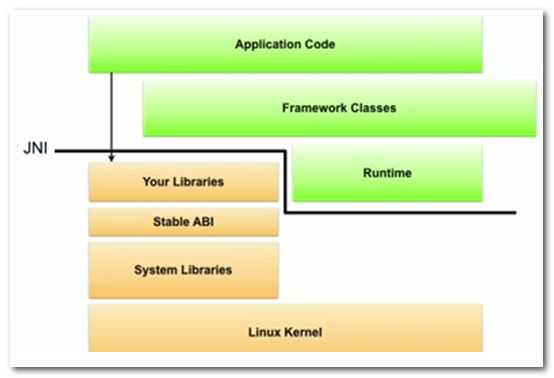
\includegraphics[width=0.8\textwidth]{images/jni.jpg}
    \caption{Android System Layer}
    \label{fig:android_application_layer}
\end{figure}

\subsection{Local Mode}
Even though the native mode reveals the terrible performance of keeping the face detection in the end devices, the computing model is not universal. In other words, a more isolated model should be used to enhance its convincingness. To be more specific, general computing task will be coded in the application layer with specific JVM supported programming languages such as Java or Kotlin but in C++ which relies on NDK to manipulate the hardware. 

To expose the data to the application layer, migration of the data from native layer to application layer is unavoidable. This process can be found in local mode, where data is transferred to the application layer before the face detection is applied.

\section{Key Sequences Diagram}
After discussing the decomposed components of the system, the blueprint of it can be view in two sequences diagrams.
The figure \ref{fig:off-peak_mode_sequence} and the figure \ref{fig:peak_mode_sequence} display the sequence diagram of the system. The first figure illustrates the sequence diagram for the off-peak mode, and the following one expresses the logic of peak mode.

\subsection{Off-peak Mode Sequence}
As you can see in the figure of \ref{fig:off-peak_mode_sequence}, there are two lifelines, namely end-devices and Fog Nodes. The initial point locates at the left side of the diagram, which is the start point of the application.

The instruction above this point says "choose computing mode". The computing mode here refers to five modes inbuilt with the android application. These five sub-modes can be observed at the bottom of the figure of \ref{fig:preview}. They are discussed in the previous sections.

The loop of processes are summarised as follows (Fog Basic and Fog DNN modes only, Native and Local modes are excluded):
\begin{enumerate}
    \item Capture previews from the camera
    \item Compress and encode the image and send the data to the Fog Node
    \item Execute Face Detection and Face Recognition according to the chosen mode
    \item Return data consist of locations of faces and related name meta-data
    \item Draw the frame on the end device
\end{enumerate}

\subsection{Peak Mode Sequence}
The figure of \ref{fig:peak_mode_sequence} displays the situation when Fog Cloud mode is activated. As the figure depicted, there is an extra lifeline compared to off-peak mode sequence. The Cloud Nodes lifeline illustrate the functionality of the cloud computing infrastructure. The comment in the diagram points out the stage where dynamic allocation algorithm is taken in part.

The loop of processes are complemented as follows (Fog Cloud Mode):
\begin{enumerate}
    \item Capture previews from the camera
    \item Compress and encode the image and send the data to the Fog Node
    \item Decide the location of the face recognition task
    \item If the load is bearable, do face recognition in the Fog Nodes
    \item If overload happens to the Fog Nodes, face recognition tasks are allocated to Cloud Nodes
    \item Return data consist of locations of faces and related name meta-data
    \item Draw the frame on the end device
\end{enumerate}

\begin{figure}
    \centering
    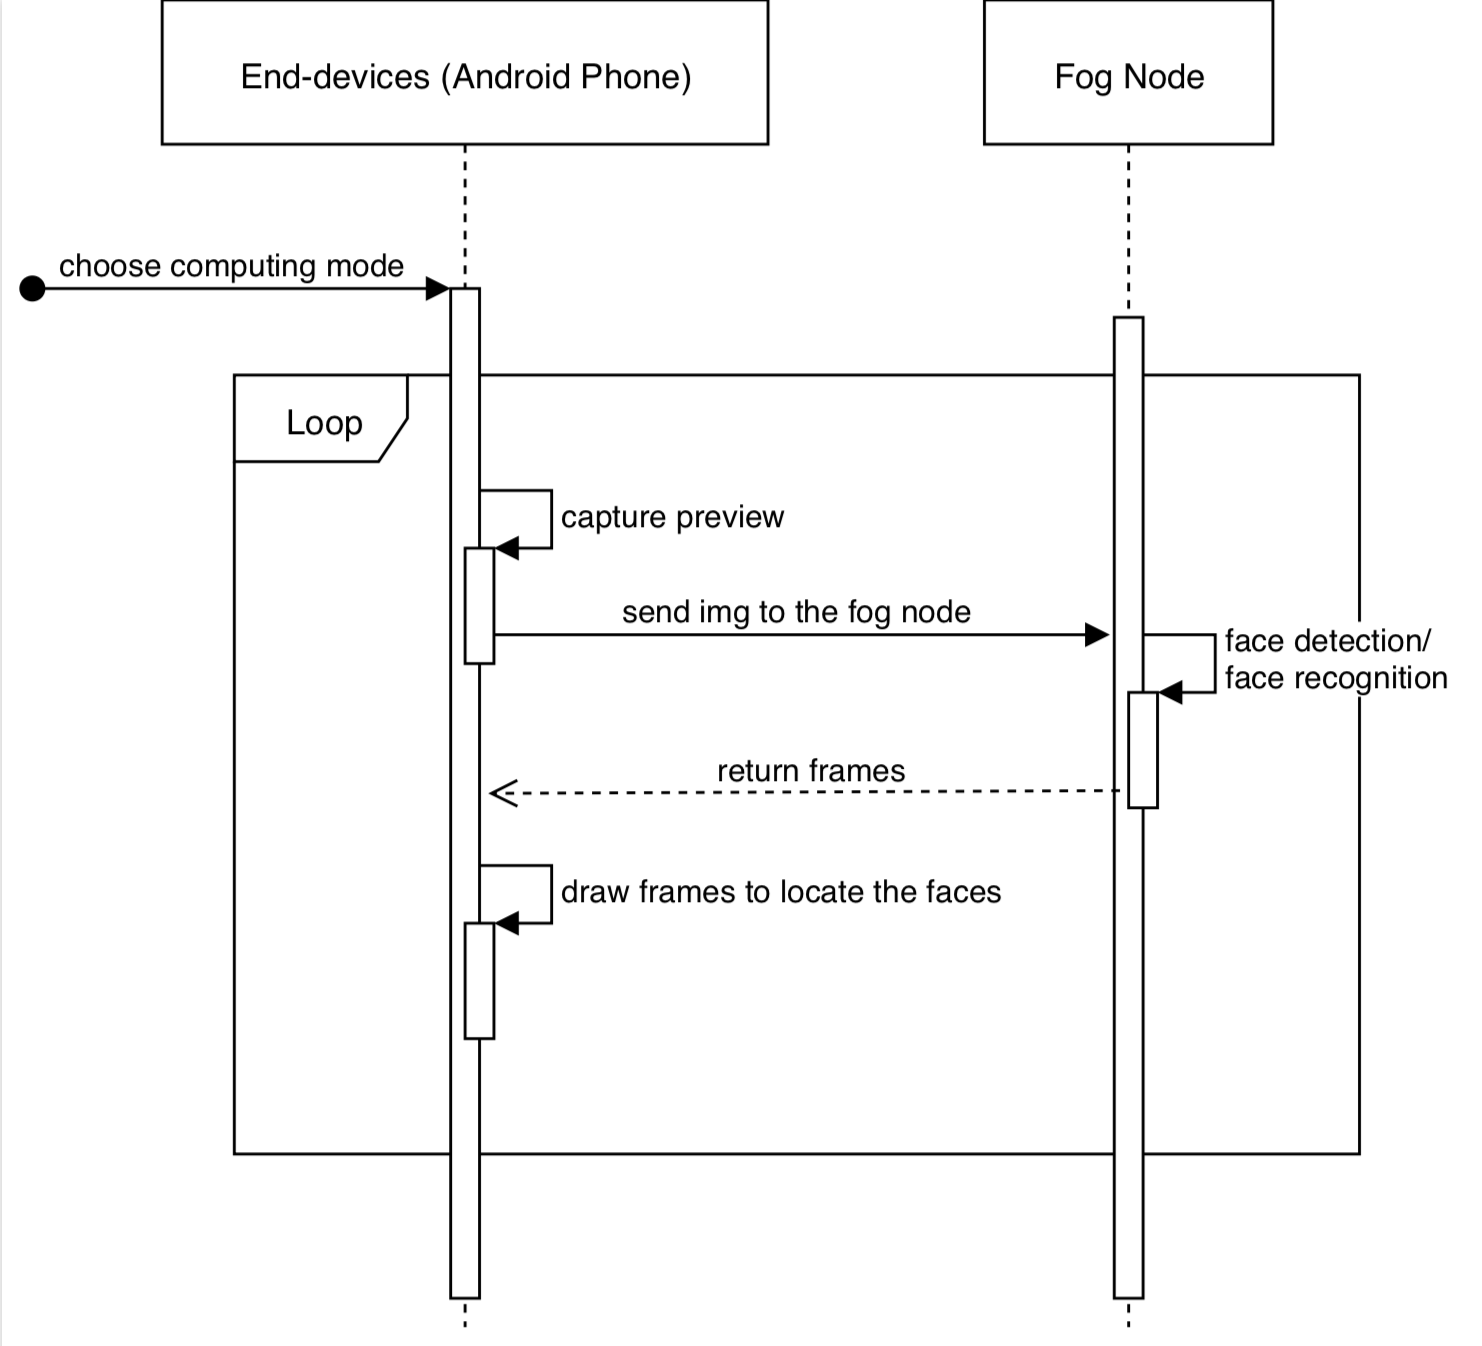
\includegraphics[width=\textwidth]{images/fog_mode.png}
    \caption{Off-peak Mode Sequence}
    \label{fig:off-peak_mode_sequence}
\end{figure}

\begin{figure}
    \centering
    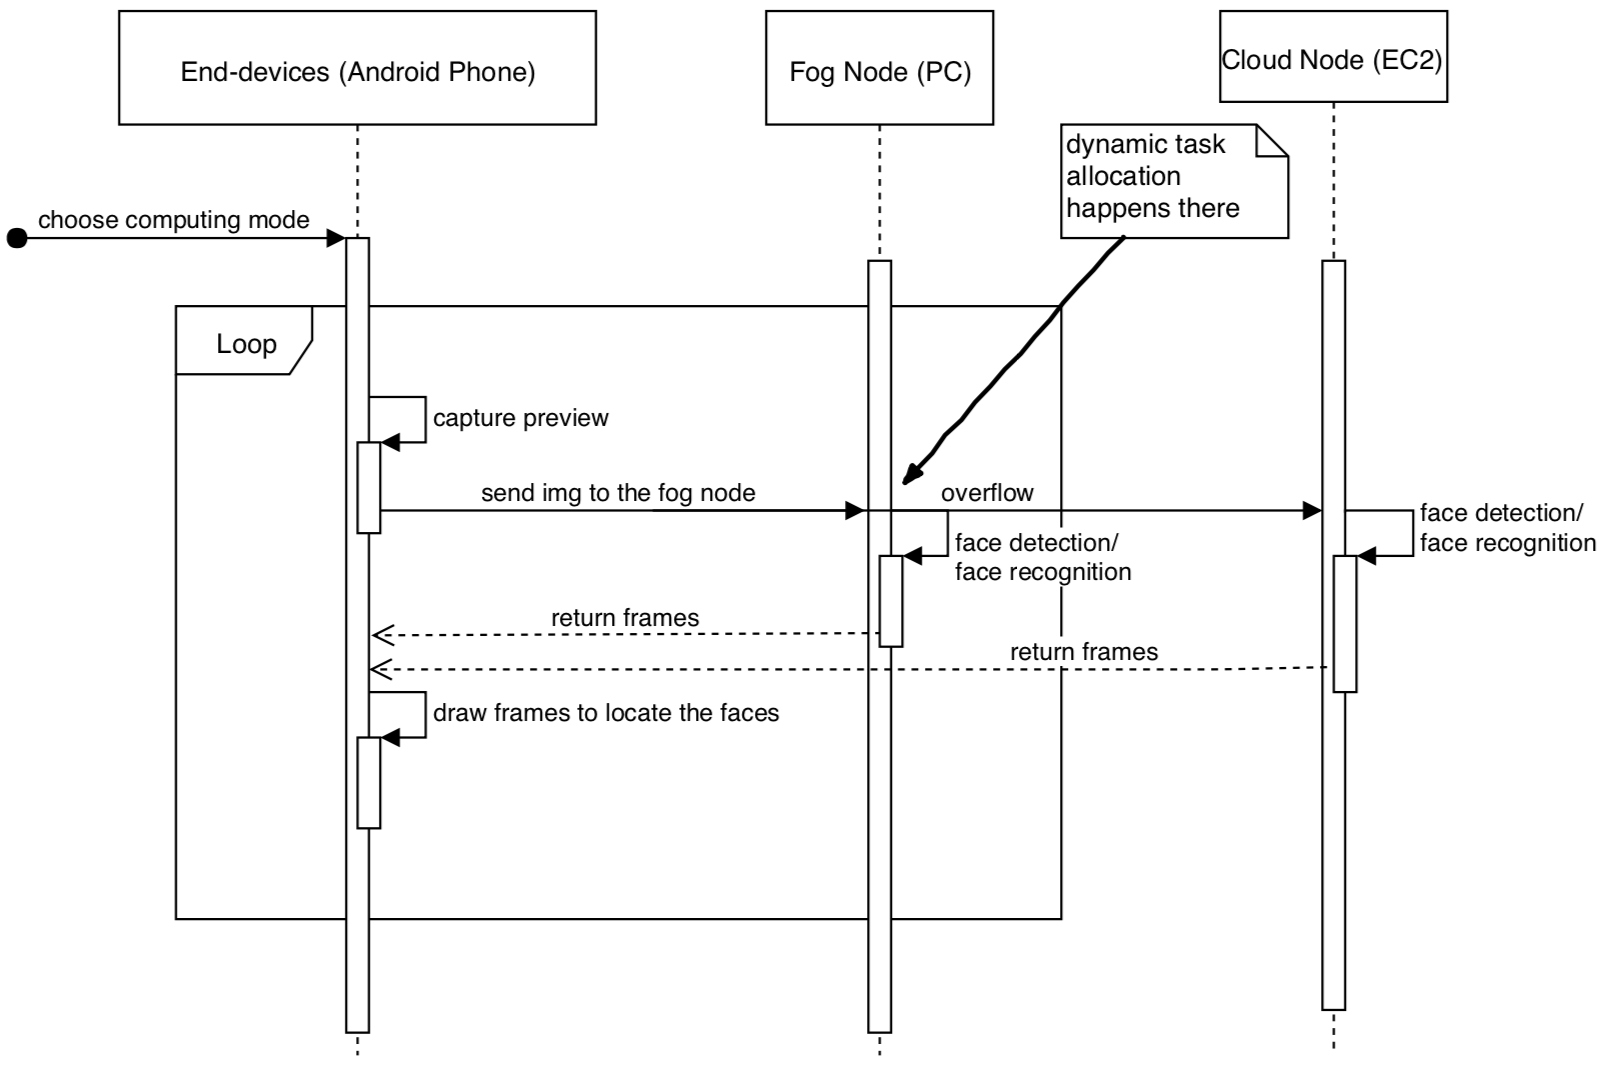
\includegraphics[width=\textwidth]{images/cloud_mode.png}
    \caption{Peak Mode Sequence}
    \label{fig:peak_mode_sequence}
\end{figure}


\begin{figure}
    \centering    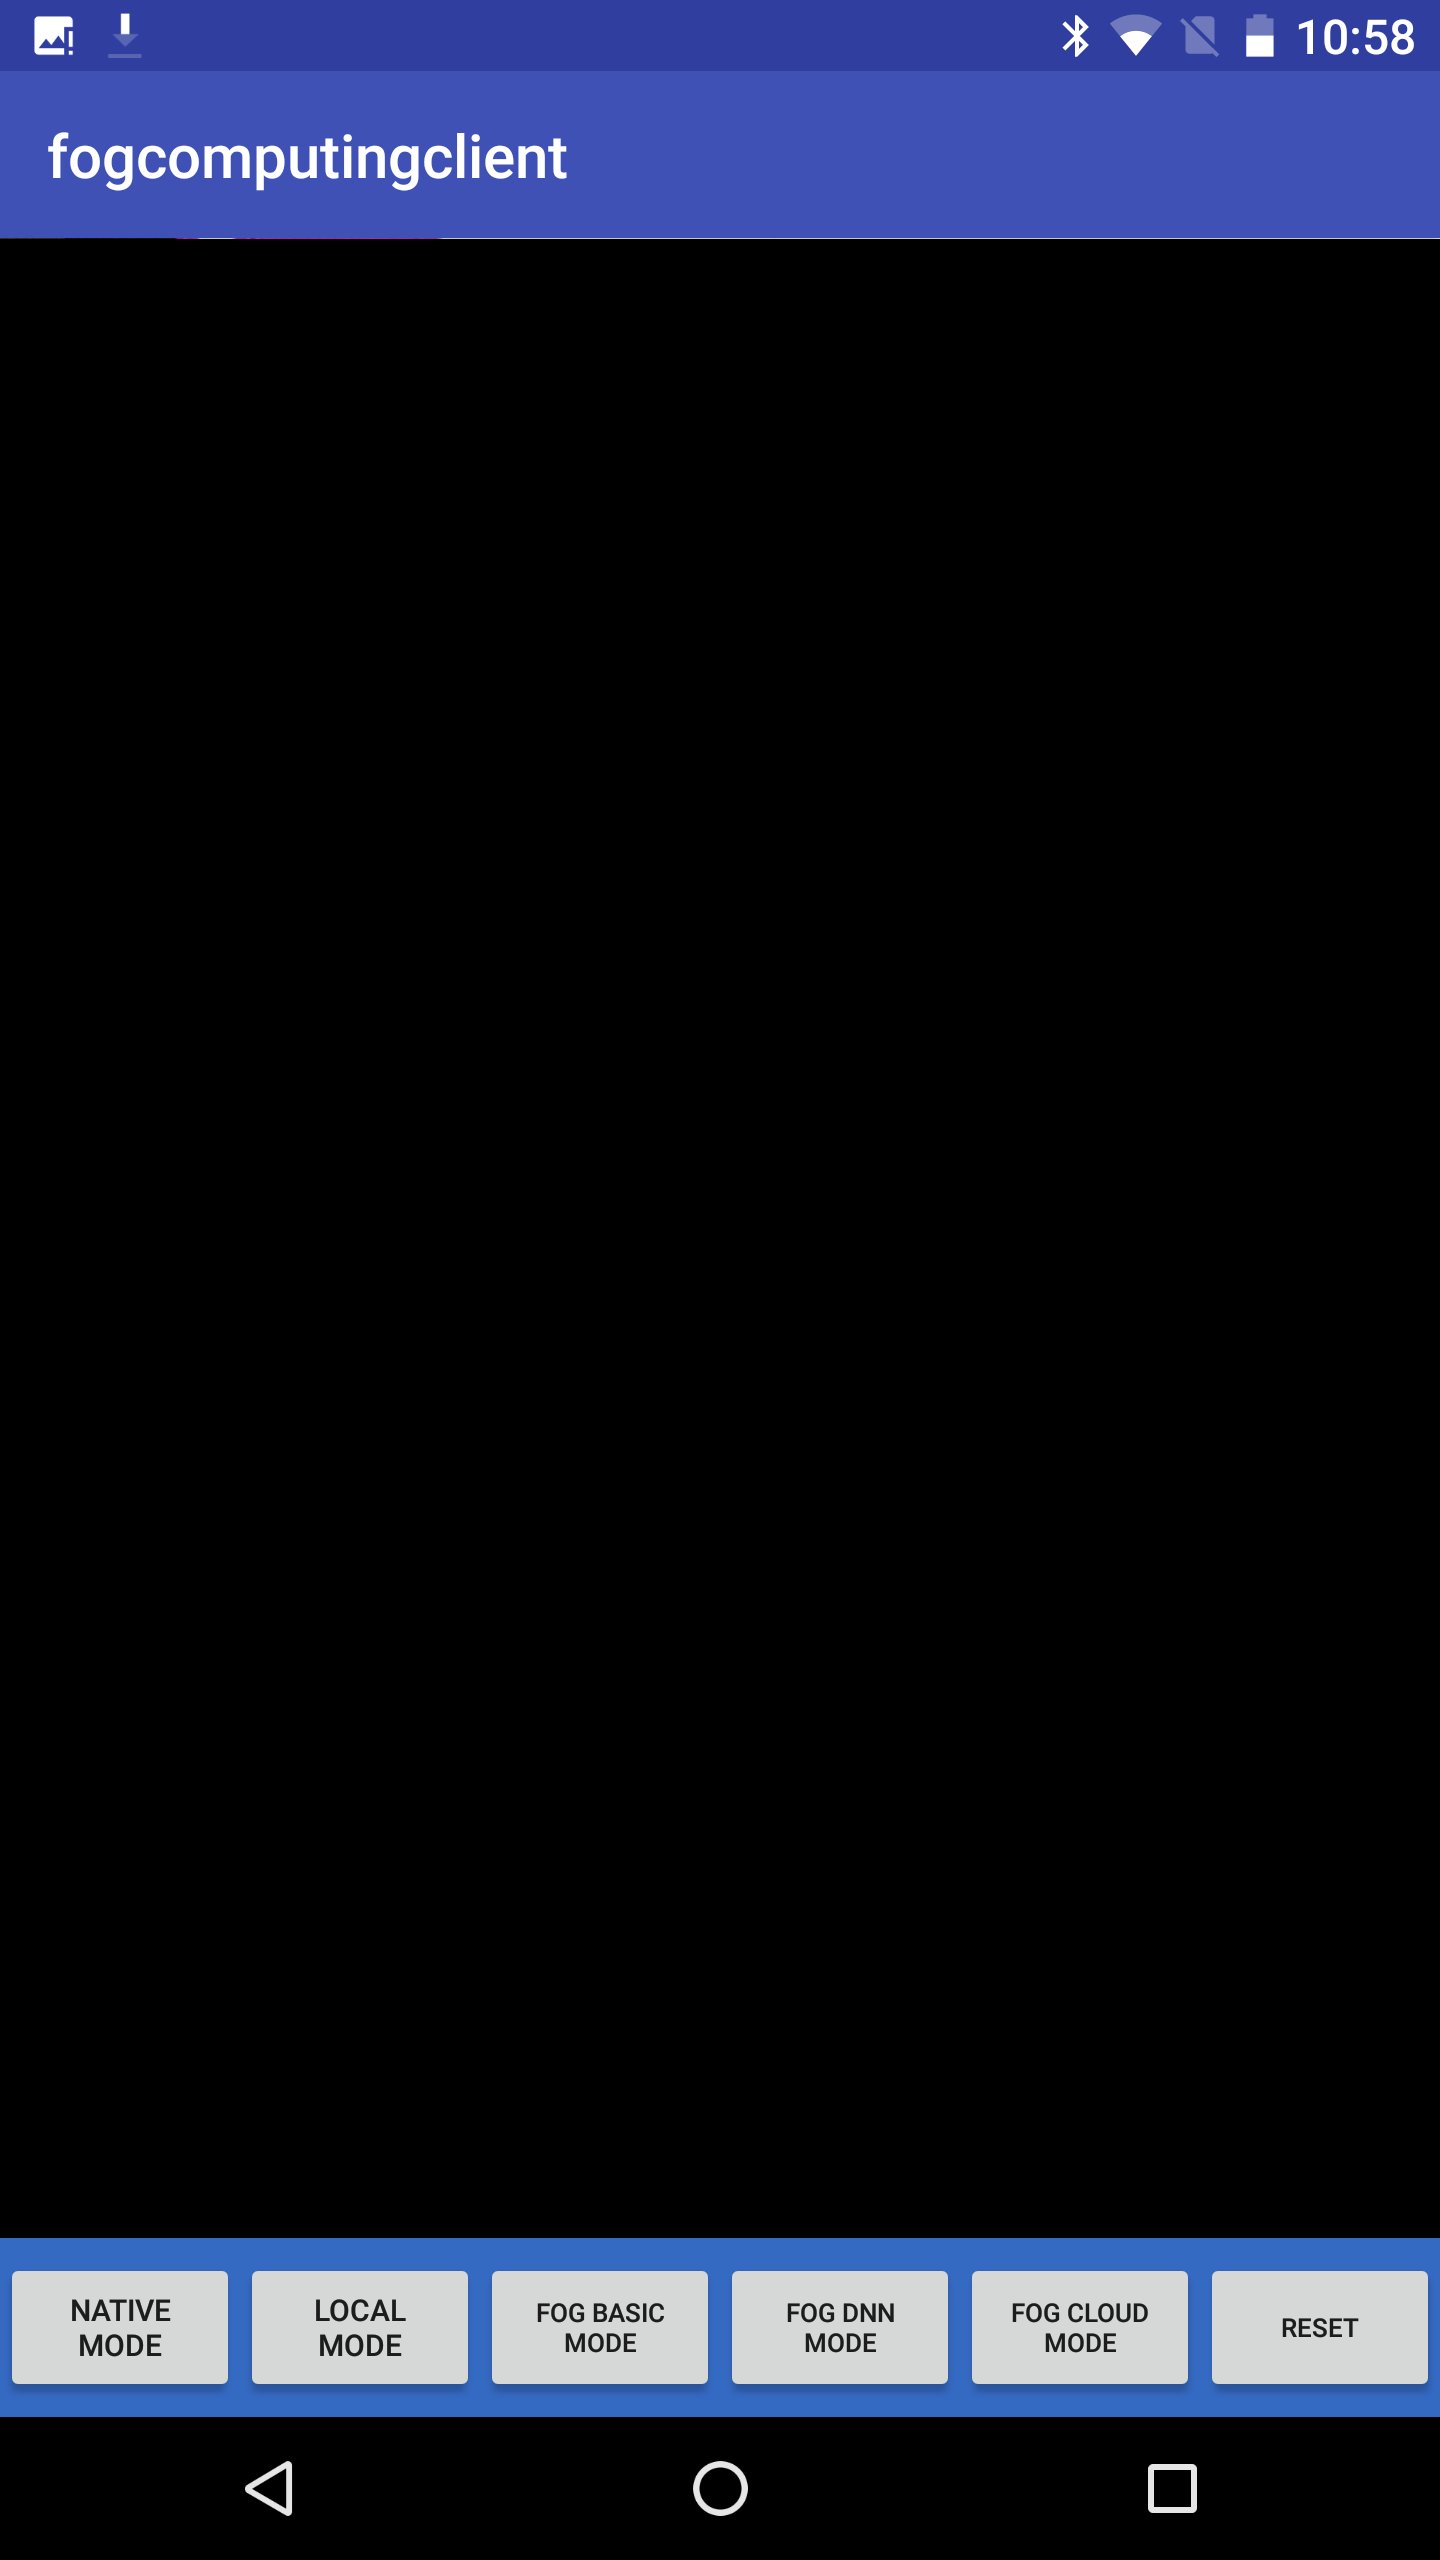
\includegraphics[width=0.6\textwidth]{images/preview.png}
    \caption{Preview of the End Devices with five modes (Android)}
    \label{fig:preview}
\end{figure}

\section{Hardware Specification}
The specification of the hardware used in the implementation can be found in the table \ref{table:end_devices_spec}, \ref{table:fog_nodes_spec} and \ref{table:cloud_nodes_spec}.

\begin{table}[ht]
\centering
\begin{tabular}{ |r|l| }
 \hline
Name &    Nexus 6\\
 \hline
Manufacturer &    Motorola Mobility\\
 \hline
Operating System &    Android 7.1\\
 \hline
Chip & Qualcomm Snapdragon 805\\
 \hline
CPU &    Qualcomm 2.7 GHz quad-core Krait 450\\
 \hline
Memory & 3 GB of LPDDR3 RAM \\
 \hline
Display & 5.96 in, 2560x1440 px, 493 ppi \\
 \hline
Front Camera & 2 MP @ 1.4um pixel \\
 \hline
Wi-Fi & 802.11 a/b/g/n/ac 2x2 (MIMO) \\
 \hline
\end{tabular}
\caption{End Devices Specification}
\label{table:end_devices_spec}
\end{table}

\begin{table}[ht]
\centering
\begin{tabular}{ |r|l| }
 \hline
Name &    PC \\
 \hline
Manufacturer &    Dell\\
 \hline
Operating System &    Ubuntu 16.04 LTS\\
 \hline
Processor & Intel Core i7-7700 CPU @ 3.60GHz x 8\\
 \hline
OS type & 64 bit\\
 \hline
Memory & 7.6 GiB\\
 \hline
\end{tabular}
\caption{Fog Nodes Specification}
\label{table:fog_nodes_spec}
\end{table}

\begin{table}[ht]
\centering
\begin{tabular}{ |r|l| }
 \hline
Name &    Amazon Web Service \\
 \hline
Instance & Various(range from t2.nano to t2 medium) \\
 \hline
Operating System &    Ubuntu 16.04 LTS\\
 \hline
Storage & Various(range from 0.5 Gib to 2 Gib)\\
 \hline
Physical Processor & Intel Xeon family\\
 \hline
Clock Speed & up to 3.3 GHz\\
 \hline
OS type & 64 bit\\
 \hline
\end{tabular}
\caption{Cloud Nodes Specification}
\label{table:cloud_nodes_spec}
\end{table}
\chapter{Performance} \label{chap:performance}
The performance of the system following the design described in the previous chapter gets discussed in the chapter. The indicators used in the measurement includes but not limited to the response time and frequency of image collection.

The result is based on the physical devices depicted in the table \ref{table:end_devices_spec}, \ref{table:fog_nodes_spec}, \ref{table:cloud_nodes_spec}. The test is conducted in the environment of the campus network in the University of Sydney. The high-speed network is supported, and the end device (Nexus 6) accesses the Fog Nodes within one hop through a wireless access point.

The performance of the Fog Basic Mode is reported firstly. The response time and the frequency of requests are the variant parameters. This benchmark aims to narrow down the exact traffic of requests that Fog Nodes are capable of handling.

As we can see in the figure \ref{fig:response_time_fog_basic}, the response time fluctuate when the frequency of face detection is relatively high. On the contrary, the response time is stable when the frequency of images collection is between 1 image per second and 0.5 images per second.


\begin{figure}
\centering
\begin{tikzpicture}
\begin{axis}[
    title={ Response Time (Fog Basic Mode)},
    xlabel={Request Sequence},
    ylabel={Response Time [millisecond]},
    xmin=1, xmax=10,
    ymin=600, ymax=3400,
    xtick={0,1,2,3,4,5,6,7,8,9,10},
    ytick={600, 800, 1000, 1200, 1400, 1600, 1800, 2000, 2200, 2400},
    legend pos=north west,
    ymajorgrids=true,
    grid style=dashed,
]
 
\addplot[
    color=orange,
    mark=square,
    ]
    coordinates {
    (1,1415)(2, 1256)(3,1902)(4,2103)(5, 1807)(6, 2105)(7, 1814)(8,2426)(9,2274)(10,2407)
    };
\addplot[
    color=blue,
    mark=oplus,
    ]
    coordinates {
    (1,1026)(2, 1179)(3,959)(4,1477)(5, 1384)(6, 1430)(7, 1499)(8,1458)(9,1518)(10,1255)
    };
 
\addplot[
    color=red,
    mark=otimes,
    ]
    coordinates {
    (1,785)(2, 748)(3,759)(4,826)(5, 800)(6, 805)(7, 847)(8,801)(9,862)(10,892)
    };
    
\addplot[
    color=cyan,
    mark=diamond,
    ]
    coordinates {
    (1,752)(2, 739)(3,764)(4,801)(5, 728)(6, 711)(7, 730)(8,843)(9,838)(10,791)
    };
    
\legend{5 images per second, 2 images per second, 1 images per second, 0.5 images per second}
\end{axis}
\end{tikzpicture}
\caption{Response Time (Fog Basic Mode)}
\label{fig:response_time_fog_basic}
\end{figure}

The statistics of the CPU usage is recorded to analyse the underlying cause of the fluctuation of the Response Time. In the figure \ref{fig:cpu_percentage_fog_basic}, the trend of CPU usage can be observed with the increasing traffic of images for face detection.

\begin{figure}
\centering
\begin{tikzpicture}
\begin{axis}[
    title={ CPU Percentage (Fog Basic Mode)},
    xlabel={Time Point},
    ylabel={CPU Percentage [\%]},
    xmin=1, xmax=10,
    ymin=0, ymax=150,
    xtick={0,1,2,3,4,5,6,7,8,9,10},
    ytick={ 20, 40, 60, 80, 100},
    legend pos=north west,
    ymajorgrids=true,
    grid style=dashed,
]
 
\addplot[
    color=orange,
    mark=square,
    ]
    coordinates {
    (1,92)(2, 79)(3,82)(4,89)(5, 90)(6, 100)(7, 100)(8,98)(9,89)(10,100)
    };
\addplot[
    color=blue,
    mark=oplus,
    ]
    coordinates {
    (1,45)(2, 53)(3,36)(4,50)(5, 54)(6, 52)(7, 59)(8,48)(9,49)(10,52)
    };
 
\addplot[
    color=red,
    mark=otimes,
    ]
    coordinates {
    (1,31)(2, 32)(3,31)(4,32)(5, 31)(6, 32)(7, 35)(8,31)(9,30)(10,32)
    };
    
\addplot[
    color=cyan,
    mark=diamond,
    ]
    coordinates {
    (1,4)(2, 9)(3,21)(4,13)(5, 18)(6, 9)(7, 8)(8,11)(9,19)(10,10)
    };
    
\legend{5 images per second, 2 images per second, 1 images per second, 0.5 images per second}
  

\end{axis}
\end{tikzpicture}

\caption{CPU Percentage (Fog Basic Mode)}
\label{fig:cpu_percentage_fog_basic}
\end{figure}


The figure \ref{fig:network_receiving_fog_basic} reveal the requirement of the precise network bandwidth. Even though campus network offers nearly unlimited bandwidth, comparing to the demand of this system, the realistic traffic deserves attention for a more confined environment in the future.

\begin{figure}
\centering
\begin{tikzpicture}
\begin{axis}[
    title={ Network Receiving (Fog Basic Mode)},
    xlabel={Time Point},
    ylabel={Receiving Rate [byte]},
    xmin=1, xmax=10,
    ymin=400, ymax=5500,
    xtick={0,1,2,3,4,5,6,7,8,9,10},
    ytick={ 600, 800, 1000, 2000, 3000},
    legend pos=north west,
    ymajorgrids=true,
    grid style=dashed,
]
 
\addplot[
    color=orange,
    mark=square,
    ]
    coordinates {
    (1,2849)(2, 3124)(3,2802)(4,3132)(5, 3454)(6, 2953)(7, 2910)(8,3011)(9,3248)(10,3350)
    };
\addplot[
    color=blue,
    mark=oplus,
    ]
    coordinates {
    (1,466)(2, 1248)(3,942)(4,962)(5, 912)(6, 972)(7, 1042)(8,1118)(9,982)(10,920)
    };
 
\addplot[
    color=red,
    mark=otimes,
    ]
    coordinates {
    (1,602)(2, 763)(3,758)(4,768)(5, 761)(6, 529)(7, 981)(8,721)(9,759)(10,811)
    };
    
\addplot[
    color=cyan,
    mark=diamond,
    ]
    coordinates {
    (1,779)(2, 776)(3,780)(4,1219)(5, 685)(6, 792)(7, 800)(8,769)(9,698)(10,780)
    };
    
\legend{5 images per second, 2 images per second, 1 images per second, 0.5 images per second}
  

\end{axis}
\end{tikzpicture}
\caption{Network Receiving on the Fog Node  (Fog Basic Mode)}
\label{fig:network_receiving_fog_basic}
\end{figure}

Table \ref{table:measure_response_time} shows the raw data sampled during the operation of the system. The data plotting line charts are generated by raw information in this format. Other raw data can be found in the appendix chapter.

The figure \ref{fig:response_time_fog_dnn} displays the outcome of the Fog DNN mode. The procedure of the test follows the same flow of sampling the response time for Fog Basic mode. Nevertheless, the gap is huge when it comes to the stable response time. From the chart, we can see the stable response time is about 5000 milliseconds. However, its counterpart in Fog Basic mode is just around 800 milliseconds. Also, the corresponding frequency is lower as well, approximately 0.2 images per second. Compared to the frequency of nearly 0.8 images per second, the delicate face recognition tasks drag the performance.

The match accuracy of the face detection and face recognition can be observed through the previews in the figure \ref{fig:preview_fog_basic} and \ref{fig:preview_fog_dnn} respectively. The face pictures are downloaded from the staff portal of the School of Information Technology in the University of Sydney.

\begin{figure}
\centering
\begin{tikzpicture}
\begin{axis}[
    title={ Response Time (Fog DNN Mode)},
    xlabel={Request Sequence},
    ylabel={Response Time [second]},
    xmin=1, xmax=10,
    ymin=0, ymax=30,
    xtick={0,1,2,3,4,5,6,7,8,9,10},
    ytick={},
    legend pos=north west,
    ymajorgrids=true,
    grid style=dashed,
]
 
\addplot[
    color=orange,
    mark=square,
    ]
    coordinates {
    (1,5.2)(2, 7.8)(3,10.29)(4,12.64)(5, 15)(17.6)(7, 20)(8,22.7)(9,24.9)(10,27.4)
    };
\addplot[
    color=blue,
    mark=oplus,
    ]
    coordinates {
    (1,4.6)(2, 5.4)(3,3.2)(4,4.5)(5, 4.7)(6, 5)(7, 5.4)(8,5.7)(9,6.1)(10,6.4)
    };
 
\addplot[
    color=red,
    mark=otimes,
    ]
    coordinates {
    (1,1.5)(2, 5.3)(3,5.1)(4,5.4)(5, 5.8)(6, 5.6)(7, 4.9)(8,5.4)(9,5.5)(10,5.5)
    };
    
\legend{ 1 image every 2 seconds, 1 image every 4 seconds, 1 image every 6 seconds,}
  

\end{axis}
\end{tikzpicture}

\caption{Response Time (Fog DNN Mode)}
\label{fig:response_time_fog_dnn}
\end{figure}
\chapter{Discussion} \label{chap:discussion}
This chapter spreads the discussion base on the performance of the implementation. The underlying logic of introducing the cloud is explained as well as the merits and demerits found in the research.

In the section of Implementation, controlled experiment setting is prepared. Though no benchmark or test against these two mode, the underperformance can be exhibited by naked eyes. For example, in the Native mode where Haar Feature-base Cascade Classifier is put into the layer of native (Yellow area in the figure \ref{fig:android_application_layer}), the performance of the application is crap. Multi-faces detection drags the render of the user interface dramatically. What's more, since the code is compiled through NDK tools, the coding work flow cannot retain consistency compared to coding in pure Java or Kotlin.

Another mode called Local mode is also included in the controlled experiment setting. The outcome of this mode is even worse due to its out of memory expectation. In this mode, the images are transferred to the application layer (Green area in the figure \ref{fig:android_application_layer}), namely Java Runtime first, then face detection is executed based it, contributing to more universal coding model. In other word, more developers or frameworks can be involved because we operate the images with Java or Kotlin code over the native layer.

The disappointing performance of previous two non-external-nodes-involved modes encourage the dependency of computing units outside. They reveal the reality that low power end devices in the network of Internet of Things have inability to handle CPU intensive tasks such as Face Detection even though the algorithm is optimised for low end hardware.

The performance of Fog Basic and Fog DNN mode are measured in the performance chapter and the difference is outstanding. Quality of the service is our initiative considering large scale deployment. If the quality of the service is acceptable, the value and reality of the system are proved.

To evaluate the quality of service, stable response time is introduced, which is the relatively constant response time by specific frequency of image collection. Frequency of image collection mimics the different pressure for the Fog Nodes in our case because the more image collected, the more face detection or recognition tasks are generated and sent to the Fog Nodes for computing. With adjusting the frequency, response time fluctuates accordingly. A thread-hold gets observed when the frequency drop to some degree, where requests with that frequency share similar response time. If you combine the result with the CPU usage, the percentage should be close to 100\% but a bit lower. So the stable response time indicate the ideal traffic of images towards that Fog Node.

The stable response time increases sharply when the face detection algorithm is replaced by face recognition algorithm, from 800 milliseconds(Fog Basic) to 5000 milliseconds(Fog DNN). Meanwhile ,the thread-hold of the traffic in Fog DNN is not ideal compared to that in Fog Basic (0.2 image per second vs 0.8 image per second). Heavy is the cost of deep metric learning supported face recognition feature.

Fog Cloud combination is the remedial solution. In the Fog Cloud mode (also called peak mode due to involvement of Cloud Nodes), unbearable tasks can be redirected to the Cloud Nodes to relief the pressure of the Fog Nodes. In this case, end devices share both benefits of Fog Nodes(low latency) and Cloud Nodes(elastic resource pool). 

In our system, the power of Cloud Nodes are assumed infinite. I achieve this goal by open sufficient AWS EC2 instances or powerful instance types ahead, so other risks are omitted currently such as orchestration of the Cloud Nodes.

Dynamic Allocation Mechanism helps judge where the requests should be assigned. The key features of it are as follows:
\begin{itemize}
    \item It calculate the capability of the Fog Node by history. (Stable response time as an indicator)
    \item It monitor the current traffic of the request and judge if Cloud Nodes are required.
    \item It overflow tasks to the Cloud Nodes by certain implementation of the proxy system.
\end{itemize}
\chapter{Conclusion} \label{chap:conclusion}

This research explains the inception of Fog Computing and discusses the appropriate scenarios based on the background of prosperous IoT devices. Accordingly, face identification attracts attention, and its computing model gets optimised in this research. Fog Computing based face identification architecture is refined after inspecting the previous related work. An aggressive model is proposed where the functionality of Fog Nodes is extended from image pre-processing to full-edged face identification.

A prototype system is implemented to evaluate the performance of the devised device-fog-cloud design. Peak and off-peak modes are composed to mimic different pressure of Fog Nodes. The performance of the Fog Basic mode (an off-peak mode) displays acceptable quality of service, offering confidence to offload face detection from Cloud. The Fog DNN mode (an off-peak mode) presents terrible outcome, leading to a dependency of the Cloud Nodes. Fog Cloud mode (peak mode) reveals the potential of a combination of Fog Nodes and Cloud Nodes where dynamic allocation mechanism is introduced to overflow tasks to Cloud Nodes in part.

Besides, the controlled experiments consisting of Native mode and Local mode, are conducted to compare the result to Fog Computing based models. In both modes, no Fog Nodes and Cloud Nodes involve. Their awkward performance strengthens the beliefs in Fog based face identification.

The combination of Fog Nodes and Cloud Nodes deliver a transparent computing model to end devices, which benefits to deploy a universal programming model. This observation is regarded as a bonus to this research.
\chapter{Future work} \label{chap:future}

go here




%%%%%%%%%%%%
% End

% Bibliography
\bibliographystyle{style/mybibstyle}
{
\setstretch{1.25}
\cleardoublepage
\phantomsection
\bibliography{references}
}

%%%% Appendices
%%%\appendix
%%%\addtocontents{toc}{\protect\setcounter{tocdepth}{1}}
%%%\input{wikifeats/wikifeats.tex}
%%%\input{candcner/candcner.tex}
%%%\input{comparedata/comparedata.tex}

\end{document}
